\documentclass[11pt,a4paper]{article}

\usepackage[margin=1.05in]{geometry}
\usepackage{amsmath,amssymb,amsthm}
\usepackage{graphicx}
\usepackage{mathtools}
\usepackage{stmaryrd}
\usepackage{booktabs}
\usepackage{listings}
\usepackage{xcolor}
\usepackage{tikz}
\usetikzlibrary{arrows.meta}
\usepackage{pgfplots}
\pgfplotsset{compat=1.16}
\usepackage[colorlinks=true,linkcolor=black,citecolor=black,urlcolor=blue]{hyperref}
\usepackage{enumitem}
\usepackage[T1]{fontenc}
\usepackage[scaled=0.92]{helvet}
\usepackage{courier}
\usepackage{mathpazo}
\usepackage[protrusion=true,expansion=false]{microtype}
\setlength{\emergencystretch}{2.5em}

%%%%%%%%%%%%%%%%%%%%%%%%%%%%%%%%%%%%%%%%%%%%%%%%%%%%%%%%%%%%%%%%%%%%%%%%%%%%%%%
% Theorem environments
%%%%%%%%%%%%%%%%%%%%%%%%%%%%%%%%%%%%%%%%%%%%%%%%%%%%%%%%%%%%%%%%%%%%%%%%%%%%%%%
\theoremstyle{plain}
\newtheorem{theorem}{Theorem}[section]
\newtheorem{proposition}[theorem]{Proposition}
\newtheorem{lemma}[theorem]{Lemma}
\newtheorem{corollary}[theorem]{Corollary}
\newtheorem{conjecture}[theorem]{Conjecture}

\theoremstyle{definition}
\newtheorem{definition}[theorem]{Definition}
\newtheorem{example}[theorem]{Example}
\newtheorem{principle}[theorem]{Principle}
\newtheorem{obligation}[theorem]{Obligation}
\newtheorem{finding}[theorem]{Empirical finding}

\theoremstyle{remark}
\newtheorem{remark}[theorem]{Remark}

%%%%%%%%%%%%%%%%%%%%%%%%%%%%%%%%%%%%%%%%%%%%%%%%%%%%%%%%%%%%%%%%%%%%%%%%%%%%%%%
% Macros.  NOTATION RULES OBSERVED THROUGHOUT:
%   * the rho calculus is never written with the Greek letter rho
%   * quoting is @P, dropping is *x; corner quotes are pre-2016 notation
%%%%%%%%%%%%%%%%%%%%%%%%%%%%%%%%%%%%%%%%%%%%%%%%%%%%%%%%%%%%%%%%%%%%%%%%%%%%%%%
\newcommand{\rhoc}{\textsf{rho}}
\newcommand{\krho}{\textsf{rho}^{\circ}}
\newcommand{\V}{\mathbb{V}}
\newcommand{\Rnn}{\mathbb{R}_{\geq 0}}
\newcommand{\Cx}{\mathbb{C}}
\newcommand{\Nat}{\mathbb{N}}
\newcommand{\scong}{\equiv}
\newcommand{\red}{\rightsquigarrow}
\newcommand{\cred}{\rightsquigarrow'}
\newcommand{\coll}{\circ}
\newcommand{\match}{\mathrm{match}}
\newcommand{\Split}{\mathrm{Split}}
\newcommand{\Frsh}{\mathsf{Fresh}_2}
\newcommand{\tr}[1]{[\![#1]\!]}
\newcommand{\loc}[2]{\langle #1,\, #2\rangle}
\newcommand{\code}[1]{\texttt{#1}}
\newcommand{\fv}{\mathrm{fv}}

\lstdefinestyle{rholang}{
  basicstyle=\ttfamily\small,
  keywordstyle=\bfseries,
  morekeywords={for,new,in,where,contract,match,if,else},
  columns=fullflexible,
  keepspaces=true,
  showstringspaces=false,
  breaklines=true,
  frame=single,
  framesep=5pt,
  rulecolor=\color{black!35},
  xleftmargin=6pt,
  aboveskip=9pt,
  belowskip=9pt
}
\lstset{style=rholang}

%%%%%%%%%%%%%%%%%%%%%%%%%%%%%%%%%%%%%%%%%%%%%%%%%%%%%%%%%%%%%%%%%%%%%%%%%%%%%%%

\title{\bfseries Collision and Scattering for Process Molecules\\[4pt]
\large Graded where-clauses beyond the well-mixed solution}

\author{L.\,G.\ Meredith\\ \small F1R3FLY.io}

\date{F1R3FLY.io working note --- October 2026\\[2pt]
\normalsize A companion to the \texttt{fuzzyware} notes on graded where-clauses}

\begin{document}
\maketitle

\begin{abstract}
The structural congruence of the rho calculus makes a large parallel
composition a multiset, and a multiset is a perfectly stirred beaker: any
receiver may meet any matching message, and nothing but multiplicity
distinguishes one configuration from another. This is exactly the
well-mixed hypothesis behind Gillespie's stochastic simulation, which the
graded where-clause already realises. This note asks what must be added if
the metaphor of a process term as a molecule is to be taken further --- far
enough to speak of bonds, of viscosity and, eventually, of turbulence.

The note records a design path and the construction it arrived at. A
\emph{location} is a splitting $\loc{K}{t}$ of a term, pointed to by
$K[t]$. A race is two terms bidding for the same location, which is a
critical pair in the sense of Knuth and Bendix. Ordinary completion would
join or orient the peak; we instead \emph{name} it. A collision is the case in
which both bidders arrive, and its outcome is a substitution produced by a
scattering kernel into the several holes of the receiver's continuation. Once
receipts may destructure their payload by pattern, the kernel need not be
primitive: matching the receiver's pattern against the parallel composite of
the arrivals is a canonical kernel, $k$-body collisions are matching against
$k$-fold composites, and the total firing rate at a site acquires a series
$\sum_k \binom{n}{k}w_k$ whose $k$-th coefficient plays the role of the $k$-th
virial coefficient. The \rhoc{} calculus is the truncation at $k=1$, the ideal
gas.

We leave receipts unmarked and count the cost. A receipt's shape decides
whether it can collide at all; the cross-section decides whether it does; and
the translation back to \rhoc{} is the identity wherever the cross-section is
zero. The translation itself --- a lock and one self-join per split of the
pattern --- is correct only after a correction we did not anticipate: each
translated candidate must be weighted by the inverse of its \emph{fibre
multiplicity}, a contingency-table count that the symmetry factor $1/k!$
alone does not capture, but which is computable locally and is therefore
admissible in a where-clause. Over $3{,}000$ random instances the corrected
translation agrees with the kernel outcome by outcome to $1.6\times10^{-15}$;
the uncorrected one overcounts by a factor of up to $24$.

Three worked examples close the note: the small kernels (association, which
is bonding; exchange; fission); collisional activation in the
Lindemann--Hinshelwood mechanism, whose fall-off curve the kernel reproduces;
and, as the example that is more than a toy, a lattice gas whose shear
viscosity is produced by the collision kernel. The two-body kernel on a square
lattice has a conserved quantity on every row and its shear wave never decays;
the two-body kernel on a hexagonal lattice still has one on every horizontal
line, and its shear wave stalls at the predicted two thirds; adding the
three-body term removes the invariant, the shear wave decays, and the measured
viscosity falls with the collision parameter, as a mean-free-path term in
$1/\lambda$ on top of a contribution from the lattice itself.
\end{abstract}

\tableofcontents

%==============================================================================
\section{Introduction}\label{sec:intro}
%==============================================================================

\subsection{The question}

In the \rhoc{} calculus the parallel composition of processes is associative
and commutative, with $0$ as unit. A population of process terms in parallel is
therefore a multiset, and it has no positions: there is no sense in which one
message is nearer to one receiver than to another. The equations were
originally intended to model a well-mixed solution, and they do so exactly.
Gillespie's derivation of the chemical master equation rests on the same
hypothesis --- reaction propensities depend on molecule counts alone --- and the
graded where-clause of the companion notes~\cite{GW,PLN,WGSLT} gives a
\rhoc{} program precisely Gillespie's semantics when the clause is valued in
$\Rnn$: candidates are counted as selections from the multiset, weighted by
the clause, and resolved as the jump chain of a continuous-time Markov
chain~\cite{Gillespie}.

But a well-mixed solution has no viscosity, no shear and no eddies. If the
metaphor of a process term as a molecule is to be taken more seriously ---
far enough to speak of bonds, of transport and eventually of turbulence --- the
calculus must say more than the multiset says. The question this note pursues is
what, minimally, must be added, and whether the graded where-clause can carry
it.

\subsection{What a fluid needs that a beaker does not}

Three things are erased by the multiset and needed by any fluid.
\emph{Position}: locality, so that only neighbours can react. \emph{Momentum}:
viscosity is the diffusion of momentum, and turbulence is a regime of a velocity
field; without a momentum carried by the molecule there is nothing for either to
be about. \emph{Time}: the graded semantics over $\Rnn$ is confined to the jump
chain (\cite{PLN}, remark ``Gillespie, precisely''), while transport coefficients live in rates.
The construction of this note supplies the second directly, gives the first a
syntactic carrier (although not, yet, an emergent one), and works with rates
throughout.

\subsection{What the note does}

Section~\ref{sec:path} records the design path: making the equations into
weighted rewrites, letting geometry emerge from interaction, and the problem
of bonding. Section~\ref{sec:locations} recasts a race as a critical pair.
Section~\ref{sec:kernel} introduces the collision kernel: two terms that race
for the same location both arrive, and their scattering is a substitution into
the receiver's holes. Section~\ref{sec:patterns} makes the kernel canonical
using destructuring patterns and derives the virial series.
Section~\ref{sec:unmarked} leaves receipts unmarked and counts the cost.
Section~\ref{sec:translation} maps the kernel back to \rhoc{} and isolates the
fibre-multiplicity correction. Section~\ref{sec:examples} gives the worked
examples, Section~\ref{sec:status} separates what is shown from what is open,
and Appendix~\ref{app:comp} documents the computations. Every number in the
note is produced by \texttt{collide.py}, which ships alongside it and uses only
the Python standard library.

\subsection{Conventions}

Quotation is $@P$ and dropping is $*x$. A send is $x!(P)$; a linear receipt is
$\code{for}(@\pi \leftarrow x)R$ and a persistent one
$\code{for}(@\pi \Leftarrow x)R$, where $\pi$ is a pattern
(Section~\ref{sec:patterns}). Structural congruence $\scong$ contains the
monoid laws for $\mid$ and $0$ and the equation $*@P \scong P$, and names are
equal when their quoted processes are congruent. In a pattern a variable $v$
matches a process $S$ and binds the \emph{name} $@S$, so the continuation
recovers the process as $*v$; this is the convention of the 2005
calculus~\cite{MeredithRadestock}, in which receipts bind names. Graded
where-clauses take
values in a commutative semiring $\V$; except where stated, $\V = \Rnn$. A
\emph{site} is a channel together with the receipts and messages on it.

%==============================================================================
\section{The design path}\label{sec:path}
%==============================================================================

The construction of Sections~\ref{sec:locations}--\ref{sec:translation} was
not the first idea, and the ideas it displaced explain its shape. This section
records them briefly.

\subsection{Two routes}

There are two ways to make a population of process terms behave like a fluid.
On the \emph{phenomenological} route viscosity is a parameter: a graded damping
on transport rates over a well-mixed or compartmentalised base, in the manner
of the reaction--diffusion master equation~\cite{Gardiner}. This is cheap and
sits within the existing machinery. On the \emph{mechanistic} route viscosity
is an output. Lattice-gas automata are the precedent~\cite{HPP,FHP,FHP87}: a
discrete rewrite system recovers the Navier--Stokes equations when its
particles carry momentum on a sufficiently symmetric lattice and its collisions
conserve mass and momentum. In that setting viscosity is computed from the
collision rules rather than put in, and turbulence appears at high Reynolds
number. This note takes the mechanistic route.

\subsection{The equations as weighted rewrites}

The path of least resistance is to stop treating the monoid equations as a
quotient and to treat them as weighted rewrites: commutativity and
associativity fire, at a rate. Mixing then becomes a process rather than an
assumption, and the well-mixed solution becomes the limit in which the
structural rewrites are infinitely fast relative to communication. Diffusion,
locality and a phenomenological viscosity (a graded clause on the swap rewrite,
by Stokes--Einstein) all follow at once.

The costs are real. The weighted-GSLT note holds that structural rules are
addressing and incur no primitive cost~\cite{WGSLT}; the unitary-equations
note places the coherent part of the dynamics in the equations~\cite{UE}, so
demoting equations to reductions moves them to the measuring side and would
decohere mixing under $\V=\Cx$. The commutativity that forces the permutation
symmetry behind the permanent in the quantum note~\cite{GWQ} is lost once
positions are distinguishable. And the geometry the oriented equations induce
is the wrong one: orienting commutativity alone gives a one-dimensional
exclusion process, in which there is no turbulence; orienting associativity as
well gives tree rotations, whose neighbourhoods are closer to hyperbolic than
Euclidean.

\subsection{Interaction means close}

The constraint the author of this note placed on the geometry is that it must
\emph{emerge from the rewrite rules}: two molecules are close to the degree
that they interact. On this reading the well-mixed solution is not a geometry
but its absence --- the complete interaction graph, of no finite dimension.
Geometry can appear only when the rewrites make interaction sparse and
repeated. Distance is then a statistic of the dynamics, such as commute-time
distance on the rate-weighted interaction graph, and dimension is read off
spectrally or from ball growth, as in the reconstruction of chromosome
conformation from contact frequencies~\cite{HiC} or the condensation of space
from a complete graph in quantum graphity~\cite{Graphity}. Viscosity acquires
an intrinsic definition as the lifetime of neighbourhoods, in the spirit of
Maxwell's relation between a liquid's viscosity and its relaxation time. This
completes, on the spatial side, the construction of~\cite{Spacetime}, where
the causal order of a spacetime is generated by the dynamics but nearness is
supplied by a contact constructor. The hazard is circularity: if closeness is
\emph{only} interaction then ``only near things interact'' is a tautology, and
something must make interaction self-reinforcing.

\subsection{Bonds}

With the restriction operator, $(\code{new}\ x)(P(x)\mid Q(x))$ is a bond, but an
unbreakable one. Scope extrusion, $(\code{new}\ x)P \mid Q \scong
(\code{new}\ x)(P\mid Q)$ when $x\notin\fv(Q)$, read as a rewrite, is bond
formation; its reverse carries the same side condition, so once $Q$ holds $x$
it can never leave, and nothing outside can ever guess $x$. The bond has
infinite binding energy. One natural way to break it is a collision that
replaces the bound name by its image under the encoding of restriction into
\rhoc{}: in the repaired encoding~\cite{NNS} that image is a quoted address
allocated by $\Frsh$, an ordinary name. Breaking the bond then changes nothing
inside $P\mid Q$ and everything about who else may reach $x$. Re-bonding is not
the inverse, since \rhoc{} cannot re-privatise a public name.

This line of thought led directly to the question of what a collision
\emph{is}, and the answer it found is the subject of the rest of the note. The
bond returns in Section~\ref{ssec:association}, where collision itself forms
one.

%==============================================================================
\section{Locations, races and critical pairs}\label{sec:locations}
%==============================================================================

\begin{definition}[Location]\label{def:location}
A \emph{location} in a term $T$ is a splitting $\loc{K}{t}$ of $T$ into a
one-hole context $K$ and a term $t$ with $K[t]\scong T$. The location is
pointed to by $K[t]$.
\end{definition}

A reduction rule acts at a location. Writing a receipt as a context, two
messages on its channel give the familiar shape
\[
P \mid K \mid Q \;\red\; K[P] \mid Q
\qquad\text{or}\qquad
P \mid K \mid Q \;\red\; P \mid K[Q] ,
\]
which does not type-check --- $K$ is a context and $P$, $Q$ are terms --- but
works as a schema for instances that do. The instance of interest is
\[
x!(P) \mid \code{for}(y\leftarrow x)R \mid x!(Q)
\;\red\; R\{@P/y\} \mid x!(Q)
\quad\text{or}\quad
x!(P) \mid R\{@Q/y\} .
\]

\begin{remark}[A race is a critical pair]\label{rem:critical}
The two redexes overlap on the receipt, so the two reducts form a critical pair
in the sense of Knuth and Bendix~\cite{KB}. The pair is not joinable, and it is
not meant to be: the race is the semantics. Completion would join the peak or
orient it into a new rule. The construction of this note does neither. It
\emph{names the peak}: a new kind of interaction is introduced for the case in
which the race is not resolved because both bidders arrive.
\end{remark}

There are two shapes of overlap. In the one displayed, two data contend for
one receipt. In the dual, $\code{for}(y\leftarrow x)R \mid x!(P) \mid
\code{for}(z\leftarrow x)S$, two receipts contend for one datum. These are the
two contention cases of the contention-set normalisation in the quantum
note~\cite{GWQ}: candidates conflict when they share a datum or a linear
receipt. This note develops the first shape, which is the one a physical
collision has, and returns to the second in Section~\ref{sec:status}.

%==============================================================================
\section{The collision kernel}\label{sec:kernel}
%==============================================================================

\subsection{Collision}

A collision is two terms racing to the same location in which, instead of one
winning, both get there, and their arrival causes an interaction. The first
form of the idea introduces an interaction term $P\coll Q$ and an augmented
reduction relation $\cred$:
\[
x!(P) \mid \code{for}(y\leftarrow x)R \mid x!(Q) \;\cred\; R[P\coll Q].
\]
As written, the right-hand side absorbs both messages and leaves nothing on
$x$. That is not scattering but \emph{association}: $P$ and $Q$ end up held
together inside $R$ by the collision. It is the bond of
Section~\ref{sec:path}, formed this time by a three-body event, and it is
recovered below as a special case.

\subsection{Scattering}

To obtain scattering, refine the interaction so that $P\coll Q$ is
multivalued, $[S_1,\dots,S_n]$, and give $R$ several holes --- these are the
locations at which the $S_i$ land. The assignment of products to holes is then
the remaining question, and it is sidestepped by letting the interaction
return the assignment itself.

\begin{definition}[Scattering kernel]\label{def:kernel}
Let $R$ have free name variables $y_1,\dots,y_n$. A \emph{scattering kernel}
for $R$ is a map $\kappa$ from pairs of processes to finite sets of
substitutions of the form $\sigma = \{@S_1/y_1,\dots,@S_n/y_n\}$. The
\emph{collision rule} is
\[
x!(P) \mid \code{for}(y_1\dots y_n \leftarrow x)R \mid x!(Q)
\;\cred\; R\sigma
\qquad (\sigma\in P\coll Q := \kappa(P,Q)),
\]
and each $\sigma$ is weighted by the receipt's graded where-clause.
\end{definition}

The collision rule has the shape of COMM. Ordinary communication yields
$R\{@P/y\}$, a substitution fixed by the match; collision yields $R\sigma$, a
substitution computed from both arrivals. So $\cred$ \emph{generalises}
communication rather than adding a new term former beside it: the scattering
is $\sigma$, and the locations are the variables. It also drops into the
graded clause unchanged. The graded clause weights candidate matches, and a
candidate match \emph{is} a substitution; if $\kappa$ returns a family of
substitutions, the clause weights them exactly as it weights any family of
candidates.

\begin{remark}[Geometry and dynamics separate]\label{rem:separate}
The receiver fixes \emph{where} products can land, through its arity and its
holes; the kernel fixes \emph{what} lands. This is how a scattering experiment
is organised --- a beam, a target, and detectors at fixed angles --- and it is
the separation that lets a later section put momentum on the holes.
\end{remark}

\subsection{Four kernels}\label{ssec:fourkernels}

\begin{example}[Association]\label{ex:assoc}
One hole, $\kappa(P,Q)=\{\{@(P\mid Q)/y\}\}$. Both arrivals end up together in
one hole.
\end{example}

\begin{example}[The race, recovered]\label{ex:race}
Two holes, with the receipt's continuation $R' = R \mid x!(*z)$, and
$\kappa(P,Q) = \{\{@P/y,@Q/z\},\{@Q/y,@P/z\}\}$. Then
$R'\{@P/y,@Q/z\} = R\{@P/y\}\mid x!(*@Q) \scong R\{@P/y\} \mid x!(Q)$, which is
the COMM reduct exactly; the ``loser'' is re-emitted exactly because
$*@Q\scong Q$. The identity kernel therefore reaches the same outcomes as the
race. It does not reach them at the same \emph{rate}: its weight adds to
COMM's, a point taken up in Section~\ref{sec:unmarked}.
\end{example}

\begin{example}[Exchange]\label{ex:exchange}
Two holes; if $P\scong A\mid B$ and $Q\scong C\mid D$, a kernel containing
$\{@(A\mid D)/y_1, @(C\mid B)/y_2\}$ exchanges parts. Elastic scattering with
exchange is crossover on quoted code.
\end{example}

\begin{example}[Fission]\label{ex:fission}
$n>2$ holes; $\kappa$ decomposes $P\mid Q$ into $n$ fragments. The holes may be
binder positions that $R$ uses or emission positions $x_i!(*y_i)$, in which
case the fragments scatter back into the medium in $n$ directions.
\end{example}

\subsection{Momentum without coordinates}\label{ssec:momentum}

Lattice-gas automata carry momentum as \emph{which outgoing direction} a
particle travels, and their collisions conserve mass and momentum by
redistributing particles among directions~\cite{FHP}. The holes of a receiver
are those directions. Label each hole $y_i$ with a direction $e_i$ and give each
process a mass $m(-)$. Conservation is then a property of the kernel:
\[
m(P) + m(Q) = \textstyle\sum_i m(S_i),
\qquad
p_{\mathrm{in}} = \textstyle\sum_i e_i\, m(S_i).
\]
Hydrodynamics needs no stated geometry beyond this --- only a kernel respecting
these constraints over a sufficiently symmetric set of holes. In graded
terms the two physical ingredients become two clause disciplines: conservation
laws are crisp guards, which zero the violating substitutions and cost
nothing~\cite{CF}; the cross-section is the graded value on the substitutions
that remain.

%==============================================================================
\section{Destructuring patterns and the canonical kernel}\label{sec:patterns}
%==============================================================================

\subsection{Patterns}

Assume term-level destructuring on the left of the arrow: in
$\code{for}(@\pi\leftarrow x)R$ the pattern $\pi$ ranges over the term
constructors of processes, some of whose arguments may be variables, together
with process variables, constants and the parallel composition of patterns.
Matching is modulo the monoid laws of $\mid$, so $\match(\pi,T)$ is a finite
\emph{set} of substitutions. A calculus with such receipts has continuations
with multiple holes by default, which removes the arity problem of
Definition~\ref{def:kernel}.

\subsection{The canonical kernel}

\begin{definition}[Canonical kernel]\label{def:canonical}
For a receipt with pattern $\pi$, the canonical $k$-body kernel is matching
against the composite of the arrivals:
\[
P_1\coll\cdots\coll P_k \;:=\; \match(\pi,\; P_1\mid\cdots\mid P_k).
\]
The kernel calculus $\krho$ has, for each $k\geq1$, the rule
\[
x!(P_1)\mid\cdots\mid x!(P_k)\mid \code{for}(@\pi\leftarrow x)R \;\red_k\; R\sigma
\qquad(\sigma\in P_1\coll\cdots\coll P_k),
\]
weighted $w_k\cdot g(\sigma)$, where $g$ is the receipt's graded where-clause
and $w_k\in\Rnn$ is the $k$-body cross-section. Persistent receipts remain.
\end{definition}

No new primitive is required: AC matching is already multivalued, so the kernel
returns a family of substitutions for free, and the receiver's pattern is the
scattering geometry --- its variables are where the products land.
$\red_1$ is COMM. The relation $\cred$ of Section~\ref{sec:kernel} is
$\bigcup_{k\geq2}\red_k$.

\begin{proposition}[The virial series]\label{prop:virial}
Let a site hold one receipt with pattern $\pi$ and messages
$x!(M_1),\dots,x!(M_n)$. The total propensity of the site is
\[
a \;=\; \sum_{k\geq1} w_k \sum_{\substack{S\subseteq\{1..n\}\\|S|=k}}
\;\sum_{\sigma\in\match(\pi,\,\prod_{i\in S}M_i)} g(\sigma).
\]
For a bare-variable pattern $\pi=y$ and $g\equiv1$ this is
$a=\sum_k \binom{n}{k}w_k$.
\end{proposition}

\begin{proof}
Candidates are counted as selections from the multiset of messages, so a
$k$-body candidate is a $k$-subset of messages together with a substitution;
the bare variable matches any composite in exactly one way.
\end{proof}

The coefficient $w_k$ plays the role of the $k$-th virial coefficient: it is the
correction that $k$-body encounters make to the ideal gas, and its contribution
grows as the $k$-th power of the occupancy. The \rhoc{} calculus is the
truncation at $k=1$. Table~\ref{tab:virial} gives the $k\leq2$ rates computed by
the generic enumerator (experiment E2).

\begin{table}[ht]
\centering
\begin{tabular}{rrrr}
\toprule
$n$ & $a$, $w_2=0$ & $a$, $w_2=0.1$ & $n + \binom n2 \cdot 0.1$ \\
\midrule
1 & 1.000 & 1.000 & 1.000\\
2 & 2.000 & 2.100 & 2.100\\
5 & 5.000 & 6.000 & 6.000\\
10 & 10.000 & 14.500 & 14.500\\
20 & 20.000 & 39.000 & 39.000\\
\bottomrule
\end{tabular}
\caption{Site propensity for a bare-variable receipt with $w_1=1$, computed by
enumerating $k$-subsets and matches.}
\label{tab:virial}
\end{table}

\subsection{The pattern decides whether a receipt can collide}

\begin{proposition}[Shape]\label{prop:shape}
Let every message payload be non-zero.
\begin{enumerate}[label=(\roman*)]
\item If $\pi$ is headed by a constructor other than $\mid$, then
$\match(\pi,P_1\mid\cdots\mid P_k)=\emptyset$ for every $k\geq2$.
\item If $\pi=\pi_1\mid\cdots\mid\pi_m$ with every $\pi_j$ headed by a
constructor other than $\mid$ (so no $\pi_j$ is a variable or matches $0$),
then $\match(\pi,P_1\mid\cdots\mid P_k) = \emptyset$ for $k>m$.
\item If $\pi$ contains a process variable at top level, the collision order
is unbounded.
\end{enumerate}
\end{proposition}

\begin{proof}
(i) A composite of $k\geq2$ non-zero processes is headed by $\mid$ up to
congruence. (ii) A composite of $k$ non-zero processes has at least $k$
top-level components, and a match distributes them among the $\pi_j$; each
$\pi_j$, being headed by a constructor other than $\mid$, absorbs exactly one.
So the composite has exactly $m$ components and $k\leq m$. (iii) A variable
absorbs any composite.
\end{proof}

So receipts stay unmarked in the syntax, but the pattern marks them. A pattern
headed by a constructor, such as $a!(u)$, is ideal-gas by construction. Only a
top-level $\mid$ or a bare variable can absorb more than one arrival, and only
a variable makes the order unbounded.

\begin{remark}[Fusion is what the pattern says]\label{rem:fusion}
A bare-variable receipt $\code{for}(y\leftarrow x)R$ says ``whatever is at this
location''. With $w_2>0$ it therefore fuses requests: two arrivals become
$\{@(P\mid Q)/y\}$. This is not a default imposed by the kernel; it is what the
pattern literally says. A program that does not want fusion writes a
constructor-headed pattern.
\end{remark}

\subsection{Conservation as a syntactic criterion}

Let the mass $m(P)$ be the number of non-zero, non-parallel components of $P$
(any additive cost measure will do).

\begin{proposition}[Mass at the pattern]\label{prop:mass}
Let $\pi = c_\pi \mid v_1 \mid \cdots \mid v_j$, with $c_\pi$ a parallel
composition of closed constants and the $v_i$ distinct variables (so $\pi$ is
linear and contains no wildcard). Then for every
$\sigma\in\match(\pi,P_1\mid\cdots\mid P_k)$,
\[
\textstyle\sum_i m(P_i) \;=\; m(c_\pi) + \sum_{v} m(*\sigma(v)),
\]
A wildcard in place of a variable discards the mass it matches. The same
accounting applies component by component to patterns whose components are
constructors with variable arguments, such as $a!(u)$.
\end{proposition}

All incoming content therefore lands either in a hole or in the pattern's
constants. Constants are absorbed by the receiver, which acts as a catalyst
unless $R$ re-emits them; for constants-only patterns, such as those of
Section~\ref{sec:examples}, conservation is the syntactic check that $R$ emits
the mass its pattern absorbs.

\begin{remark}[Bound and collided look the same]\label{rem:bound}
One message $x!(A\mid B)$ and two messages $x!(A)$, $x!(B)$ produce the same
substitution. A receiver cannot tell a pre-bonded molecule from a collision
complex; only the rates differ, first order against second. Physically this may
be right --- the location holds the same stuff --- but it means a bond is visible
only kinetically, never structurally. A collision constructor in the pattern
language would distinguish the two at the cost of a new pattern former.
\end{remark}

%==============================================================================
\section{Unmarked receipts}\label{sec:unmarked}
%==============================================================================

Should the kernel mark collision-capable receivers in its syntax? Marking keeps
the translation local and makes the identity on \rhoc{} trivial; leaving
receipts unmarked is closer to physics, in which every molecule can collide. We
leave them unmarked and count the cost.

\begin{proposition}[The ideal gas]\label{prop:ideal}
If $w_k=0$ for all $k\geq2$, the outcome-weighted semantics of $\krho$ is that
of graded \rhoc{}, outcome by outcome.
\end{proposition}

\begin{proof}
Only $\red_1$ has non-zero weight, and $\red_1$ is COMM.
\end{proof}

Experiment E2 confirms the statement on $2{,}000$ random instances with
discrepancy exactly $0$. Marking therefore returns, but semantically: a
receipt with zero cross-section is a receipt of the ideal gas, and the
translation of Section~\ref{sec:translation} will be the identity on it. The
costs of the unmarked choice are the following.

\paragraph{Kinetics change, and sometimes support.}
For the identity kernel of Example~\ref{ex:race} collisions reach only COMM
outcomes, so crisp support survives; for the canonical kernel a pattern that
can absorb several arrivals reaches new outcomes as well
(Remark~\ref{rem:fusion}). In either case, under $\V=\Rnn$ collision weight
adds to the propensity of a site, and it adds superlinearly in occupancy. Within one site this reweights outcomes; across
sites it reweights the jump chain, boosting crowded sites
(Table~\ref{tab:jump}). Rates are conserved only in the limit $w_k\to0$ for
$k\geq2$, or equivalently the dilute limit. This is physically correct: it is
the departure of a real gas from an ideal one as density grows.

\begin{table}[ht]
\centering
\begin{tabular}{rcc}
\toprule
$w_2$ & P(site with 2 messages fires) & P(site with 20 messages fires)\\
\midrule
0.00 & 0.090909 & 0.909091\\
0.01 & 0.084065 & 0.915935\\
0.10 & 0.051095 & 0.948905\\
1.00 & 0.014085 & 0.985915\\
\bottomrule
\end{tabular}
\caption{Jump-chain probability of the next firing, two bare-variable sites,
$w_1=1$.}
\label{tab:jump}
\end{table}

\paragraph{The translation gets expensive.}
Every collidable receipt acquires a lock and a family of self-joins
(Section~\ref{sec:translation}); a persistent receipt needs a fresh lock at
every firing, so the cost-accounted translation charges one $\Frsh$ rendezvous
per firing. Joins compound it: in a $k$-way join each component could collide
independently, giving $2^k$ branches, which the dilute approximation --- at most
one collision per firing --- reduces to $k+1$.

\paragraph{Unbounded order.}
By Proposition~\ref{prop:shape}(iii) a pattern with a top-level process
variable admits collisions of every order. The series of
Proposition~\ref{prop:virial} does not stop and the translation would be
infinite. A truncation order $K$ is required; it is the dilute-gas
approximation, stated as a parameter.

\paragraph{The coherent instance breaks.}
Under $\V=\Cx$ the one-body and $k$-body branches \emph{interfere} wherever
they reach the same outcome, so every communication acquires a phase-sensitive
correction and can be cancelled outright. This note is scoped to $\Rnn$.

\paragraph{What unmarked buys.}
There is no marking to preserve under reduction. The choice-formulae note shows
that a static annotation can be mailed in through reflection: a received
process dropped by $*y$ brings its own receipts into the receiver's
code~\cite{CF}. With every receipt treated alike, that is not an issue.

%==============================================================================
\section{The map back to rho}\label{sec:translation}
%==============================================================================

The presentation is a kernel that makes the intuitions clear, followed by a map
from the kernel back to \rhoc{} without it. The ordinary branch and the
collision branches must compete for the same messages, and \rhoc{} has no
summation, so each receipt becomes a family of atomic joins sharing a lock.

\subsection{Splitting a pattern across arrivals}

In a $k$-fold self-join each join component sees one message, so the pattern
must be split across the arrivals. A variable may \emph{straddle}: in
$\match(\pi, P\mid Q)$ a variable $u$ may bind $A\mid B$ with $A$ drawn from
$P$ and $B$ from $Q$.

\begin{definition}[Split]\label{def:split}
A $k$-split of $\pi = c_\pi \mid v_1\mid\cdots$ assigns each occurrence of a
constant in $c_\pi$ to one of $k$ components and replaces each variable $v$ by
fresh variables $v^1,\dots,v^k$, one per component. Component $i$ is the pattern
$\pi^s_i = c^s_i \mid v_1^i\mid\cdots$. $\Split_k(\pi)$ is the set of $k$-splits;
for a pattern whose constants have multiplicities $c_a$ it has
$\prod_a\binom{c_a+k-1}{k-1}$ elements.
\end{definition}

\begin{lemma}[Recombination]\label{lem:recombine}
Let $\theta_v := @(*v^1\mid\cdots\mid *v^k)$. If $v^i$ is bound to $@S^i$ then
$\theta_v$ becomes $@(S^1\mid\cdots\mid S^k)$.
\end{lemma}

\begin{proof}
Substitution gives $@(*@S^1\mid\cdots\mid *@S^k)$, and $*@S\scong S$ inside the
quote, since names are equal when their quoted processes are congruent.
\end{proof}

The equation $*@P\scong P$ therefore carries the correctness of the
translation.

\subsection{The translation}

\begin{definition}[Translation]\label{def:translation}
For a linear receipt and truncation order $K$,
\[
\begin{aligned}
\tr{\code{for}(@\pi\leftarrow x)R}_K \;=\;
\code{new}\ l\ \code{in}\ \Big(\, l!(0) \;\Big|\;
&\prod_{k=1}^{K}\ \prod_{s\in\Split_k(\pi)}
\code{for}(@\pi^s_1\leftarrow x \,\&\cdots\&\, @\pi^s_k\leftarrow x\\
&\qquad\qquad\,\&\, \_\leftarrow l\ \code{where}\ \omega_{k})\; R\{\theta_v/v\}_v \Big),
\end{aligned}
\]
with clause value
\[
\omega_k \;=\; \frac{w_k\, g(\sigma)}{\mu(P_1,\dots,P_k;\sigma)},
\]
where $\sigma$ is the recombined substitution and $\mu$ is the fibre
multiplicity of Definition~\ref{def:mu}. The lock is allocated by $\Frsh$ when
the target is \rhoc{} without restriction~\cite{NNS}. A persistent receipt
reinstalls its lock, freshly allocated, at every firing.
\end{definition}

Atomic joins remove the partial-commitment problem that defeats encodings of
guarded choice through a lock, since a join commits all at once. Gillespie's
selection counting then gives the $k$-body branches their combinatorics
automatically: the second-order kinetics of collision are a consequence of the
translation, not a stipulation. The losing branches are left blocked on a
consumed private lock; they are behaviourally inert, but correctness is stated
up to this garbage.

\subsection{The fibre multiplicity}

The naive expectation is that each translated candidate should carry the
kernel's weight $w_k g(\sigma)$, perhaps divided by the symmetry factor $k!$
for the orderings of the join. Both are wrong. A single kernel outcome is
reached by many translated candidates: every ordering of the $k$ messages,
every split, and every decomposition of each straddling variable's binding
across the components. When atoms are indistinguishable, several splits reach
the same outcome.

\begin{definition}[Fibre multiplicity]\label{def:mu}
For messages $P_1,\dots,P_k$ and an outcome $\sigma$, let $n_{i,a}$ be the
number of occurrences of atom $a$ in $P_i$, $c_a$ that in $c_\pi$, and
$s_{v,a}$ that in $*\sigma(v)$. Let $T_a$ be the number of non-negative integer
matrices with rows indexed by $i$, columns indexed by the roles
$\{c\}\cup\{v\}$, row sums $n_{i,a}$ and column sums $(c_a, s_{v,a},\dots)$. Then
\[
\mu(P_1,\dots,P_k;\sigma) \;=\; k!\,\prod_a T_a .
\]
\end{definition}

\begin{theorem}[Correspondence]\label{thm:corr}
Fix a site and a truncation order $K$. For every outcome --- a set of consumed
messages together with a substitution --- the total weight assigned by the
translation equals the weight $w_k g(\sigma)$ assigned by $\krho$.
\end{theorem}

\begin{proof}[Proof sketch]
Translated candidates reaching a fixed outcome are in bijection with pairs of
an ordering of the consumed messages and, for each atom type, a matrix
distributing the occurrences of that atom in each message among the roles; a
matrix is admissible exactly when its column sums reproduce the outcome. There
are therefore $\mu$ of them, each weighted $w_kg(\sigma)/\mu$. Conversely every
kernel outcome is reached from every ordering, because $\pi\sigma\scong
P_1\mid\cdots\mid P_k$ makes each $P_i$ a sub-multiset of $\pi\sigma$.
\end{proof}

\begin{remark}[$\mu$ is admissible]\label{rem:local}
$\mu$ depends only on the messages a candidate consumes and on its own
bindings, both of which a where-clause sees. The correction is therefore
expressible in the target, and the translation stays within graded \rhoc{}.
It is the outcome-fibre normalisation of the quantum note~\cite{GWQ} met again
in a different setting: weights must be summed over the fibre of an outcome,
not over the derivations that reach it.
\end{remark}

\begin{finding}[E1]\label{find:e1}
Over $3{,}000$ random sites ($1{,}820$ with a non-empty kernel), with up to four
messages over three atom types, patterns with up to two constants and two
variables, and $K=3$:
\begin{itemize}[nosep]
\item with weight $w_kg/\mu$ the translation agrees with the kernel outcome by
outcome, worst relative discrepancy $1.6\times10^{-15}$, with identical
supports; the largest multiplicity met is $\mu=108$;
\item with weight $w_kg/k!$ the total weight is overcounted by a factor of
$1.281$ on average and up to $5.162$;
\item with weight $w_kg$ the overcount is $3.639$ on average and up to
$24.32$.
\end{itemize}
\end{finding}

\begin{proposition}[Identity at zero cross-section]\label{prop:identity}
If $w_k=0$ for $k\geq2$ the lock and all collision branches may be omitted,
and $\tr{\code{for}(@\pi\leftarrow x)R}_K = \code{for}(@\pi\leftarrow x)R$.
In particular the translation is the identity on every \rhoc{} program whose
receipts have zero cross-section.
\end{proposition}

\begin{proof}
With a single branch the lock never decides anything, and $\mu=1$ for $k=1$.
\end{proof}

%==============================================================================
\section{Worked examples}\label{sec:examples}
%==============================================================================

\subsection{Small kernels}\label{ssec:association}

\paragraph{Association is bonding.}
The receipt
\begin{lstlisting}
for( @y <- x ){ bound!( *y ) }
\end{lstlisting}
with $w_2>0$ turns two arrivals $x!(P)$, $x!(Q)$ into $\code{bound}!(P\mid Q)$:
$P$ and $Q$ now travel together. Unlike $(\code{new}\ z)(P\mid Q)$ the bond is
breakable, by a dissociation receipt whose pattern recognises the parts:
\begin{lstlisting}
for( @(a!(u) | b!(v)) <= bound ){ x!( a!(*u) ) | x!( b!(*v) ) }
\end{lstlisting}
By Remark~\ref{rem:bound} the receiver on \code{bound} cannot tell a bound pair
from a pair that happens to arrive together; it sees the same substitution, at a
different rate.

\paragraph{Exchange.}
Molecules are pairs $\code{left}!(A)\mid\code{right}!(B)$. The receipt
\begin{lstlisting}
for( @( left!(u1) | right!(u2) | left!(u3) | right!(u4) ) <- x ){
  x!( left!(*u1) | right!(*u4) ) | x!( left!(*u3) | right!(*u2) )
}
\end{lstlisting}
cannot fire on one message, which has two parts against a four-part pattern
(Proposition~\ref{prop:shape}(ii)); it is a collision-only receipt. On two
messages AC matching returns four substitutions, according to which
\code{left} is bound to \code{u1} and which \code{right} to \code{u2}. Two of
them return the input pair unchanged (elastic scattering without exchange) and
two exchange partners; the graded clause decides the ratio. Mass is conserved:
the pattern is linear and wildcard-free, and the four sends it absorbs are
re-emitted as four sends.

\paragraph{Fission.}
\begin{lstlisting}
for( @(u1 | u2 | u3) <- x ){ x1!( *u1 ) | x2!( *u2 ) | x3!( *u3 ) }
\end{lstlisting}
scatters the content of the arrivals in three directions. Its pattern has
top-level process variables, so by Proposition~\ref{prop:shape}(iii) its
collision order is unbounded and a truncation order must be chosen.

\subsection{Collisional activation: Lindemann--Hinshelwood}

A molecule $A$ cannot decompose until a collision with a bath molecule $M$
has activated it~\cite{Lindemann,Hinshelwood}. On one location $x$ the laws are
four persistent receipts:
\begin{lstlisting}
for( @(A | M)  <= x ){ x!(Astar) | x!(M) }   // activation,   k = 2, weight k1
for( @(Astar | M) <= x ){ x!(A) | x!(M) }    // deactivation, k = 2, weight km1
for( @Astar <= x ){ x!(B) }                  // decomposition, k = 1, weight k2
for( @B <= x ){ x!(A) }                      // recycling,     k = 1, weight r
\end{lstlisting}
The first two patterns are constants-only with two components, so by
Proposition~\ref{prop:shape}(ii) they fire only as two-body collisions, and the
generic enumerator gives them propensity $k_1n_An_M$ and $k_{-1}n_{A^*}n_M$
(experiment E3: $400$ random site configurations, discrepancy $0$). In the ideal
gas, $w_2=0$, activation is impossible: the pattern $A\mid M$ matches no single
message. In plain rholang one would have written the join
$\code{for}(@A\leftarrow x\ \&\ @M\leftarrow x)$, and that is precisely what the
translation of Section~\ref{sec:translation} produces.

Each molecule of $A$ moves independently among $A$, $A^*$ and $B$, so the
effective unimolecular rate constant $k_{\mathrm{uni}} = J/\langle n_A\rangle$
satisfies the Lindemann law exactly:
\[
k_{\mathrm{uni}} \;=\; \frac{k_1k_2\,n_M}{k_{-1}n_M + k_2},
\]
second order ($k_1n_M$) at low bath density, where collisions limit the rate,
and first order ($k_1k_2/k_{-1}$) at high density, where decomposition does.
Table~\ref{tab:lindemann} gives the fall-off curve measured by stochastic
simulation of the kernel.

\begin{table}[ht]
\centering
\begin{tabular}{rcccc}
\toprule
$n_M$ & $k_{\mathrm{uni}}$ measured & exact & low-density limit & high-density limit\\
\midrule
1 & $0.907\pm0.005$ & 0.909 & 1.0 & 10.0\\
3 & $2.309\pm0.016$ & 2.308 & 3.0 & 10.0\\
10 & $4.981\pm0.019$ & 5.000 & 10.0 & 10.0\\
30 & $7.538\pm0.061$ & 7.500 & 30.0 & 10.0\\
100 & $9.053\pm0.163$ & 9.091 & 100.0 & 10.0\\
300 & $9.810\pm0.150$ & 9.677 & 300.0 & 10.0\\
1000 & $9.862\pm0.116$ & 9.901 & 1000.0 & 10.0\\
\bottomrule
\end{tabular}
\caption{Fall-off of the unimolecular rate with bath density. $k_1=k_{-1}=1$,
$k_2=10$, $r=50$, $50$ molecules of $A$; each measurement is the mean $\pm$
standard deviation of three runs of $10{,}000$ decompositions.}
\label{tab:lindemann}
\end{table}

\subsection{A lattice gas whose viscosity comes from the kernel}\label{ssec:lattice}

This is the example that is more than a toy. A shear wave is a sinusoidal
profile of $x$-momentum varying in $y$; in a fluid it decays as
$e^{-\nu k^2t}$, and the decay rate measures the kinematic viscosity $\nu$. We
write a lattice gas in $\krho$, measure $\nu$, and find that it is produced by
the collision kernel --- and that the kernel's two-body term is not enough.

\paragraph{The program.}
Sites are channels $s$ on an $L\times L$ torus; a particle moving in direction
$d$ is a message $s!(p_d)$. At every site the laws are
\begin{lstlisting}
for( @p_d <= s ){ (s + e_d)!(p_d) }                          // stream, k = 1, h
for( @(p_d | p_{d+3}) <= s ){ s!(p_{d+1}) | s!(p_{d+4}) }    // pair,  k = 2, w2/2
for( @(p_d | p_{d+3}) <= s ){ s!(p_{d-1}) | s!(p_{d+2}) }    // pair,  k = 2, w2/2
for( @(p_0 | p_2 | p_4) <= s ){ s!(p_1) | s!(p_3) | s!(p_5) } // triple, k = 3, w3
for( @(p_1 | p_3 | p_5) <= s ){ s!(p_0) | s!(p_2) | s!(p_4) } // triple, k = 3, w3
\end{lstlisting}
with six directions $e_d$ at angles $60^\circ d$ on a hexagonal lattice (FHP,
\cite{FHP}), indices mod $6$. The square-lattice variant (HPP, \cite{HPP}) has
four directions and the pair law $(E,W)\leftrightarrow(N,S)$. Unlike the
classical automata the model is asynchronous, in continuous time, and without
exclusion: a site may hold any number of particles in each direction. Geometry
here is supplied by the namespace --- the site names --- not grown from
interaction; Section~\ref{sec:status} returns to this.

All collision patterns are constants-only, so the collision orders are fixed
($k=2$ and $k=3$) by Proposition~\ref{prop:shape}(ii), the propensities are
$\tfrac{w_2}{2}n_dn_{d+3}$ per rotation and $w_3n_0n_2n_4$, $w_3n_1n_3n_5$
(experiment E3, discrepancy $0$), and every law conserves mass and momentum:
a head-on pair and its rotation both have zero momentum, as do the two triples
of directions $120^\circ$ apart.

\begin{proposition}[Line invariants]\label{prop:lines}
\begin{enumerate}[label=(\roman*)]
\item In the HPP kernel the quantity $\sum_{s\in r}(n_E(s)-n_W(s))$ is
invariant for every row $r$.
\item In the FHP kernel with $w_3=0$, for every horizontal line $r$ the quantity
$\sum_{s\in r}(n_0(s)-n_3(s))$ is invariant.
\item The triple laws change $n_0-n_3$ by $\mp2$ at a site, so for $w_3>0$
statement (ii) fails.
\end{enumerate}
\end{proposition}

\begin{proof}
A pair collision removes one particle from each of two opposite directions and
adds one to each of two others, so it preserves every difference
$n_d-n_{d+3}$. Particles in directions $0$ and $3$ (HPP: $E$ and $W$) stream
along their line and never leave it; no other direction contributes to the
difference. For (iii), $(0,2,4)\to(1,3,5)$ removes a $0$ and adds a $3$.
\end{proof}

In the initial condition used here the occupation of direction $d$ at line $r$
is Poisson with mean $f(1 + a\cos(60^\circ d)\sin(2\pi r/L))$ (for HPP,
$f(1 + 2a\cos(90^\circ d)\sin(2\pi r/L))$). The observable is
the projected $x$-momentum $A(t)=\sum_{s,d} n_d(s)\cos(60^\circ d)
\sin(2\pi r(s)/L)$, whose expected initial value is proportional to
$fa\sum_d\cos^2(60^\circ d) = 3fa$. Directions $0$ and $3$ contribute $2fa$
of it, so Proposition~\ref{prop:lines}(ii) predicts that without triple
collisions the shear wave can decay to no less than $\tfrac23$ of its initial
amplitude. For HPP the whole of $A$ is invariant.

\begin{finding}[E5, invariants]\label{find:plateau}
With $L=16$, $f=2$, $a=\tfrac12$ and six runs averaged, the mean of $A(t)/A(0)$
over the second half of a run of length $60$ is
\begin{center}
\begin{tabular}{lc}
\toprule
kernel & late-time $A/A(0)$\\
\midrule
HPP, pairs ($w_2=1$) & 1.0000\\
FHP, no collisions (ideal gas) & 0.6470\\
FHP, pairs only ($w_2=1$, $w_3=0$) & 0.6556\\
FHP, pairs and triples ($w_2=1$, $w_3=\tfrac12$) & 0.1674\\
\bottomrule
\end{tabular}
\end{center}
against the predicted $1$ for HPP and $\tfrac23$ for FHP without triples.
\end{finding}

The HPP value is exact because the whole observable is a sum of line
invariants. The FHP ideal gas sits at the same two thirds as the pair kernel
for a different reason: without collisions the particles in the four oblique
directions keep their directions, and the randomness of asynchronous streaming
spreads and dephases their contribution, while directions $0$ and $3$ never
leave their lines. Two-body collisions, which are what a reader would write
first, therefore buy nothing for this mode: they relax every oblique
contribution that free streaming would have dephased anyway, and leave the
invariant untouched. The three-body term --- the third virial coefficient of
Proposition~\ref{prop:virial} --- is what makes the shear wave decay. In the
language of the lattice-gas literature this is the familiar observation that
pair collisions alone leave spurious conservation laws, and that triple
collisions are added to FHP to remove them~\cite{FHP87}; here it appears as a
statement about which terms of the virial series a kernel keeps.

\paragraph{Viscosity.}
With pair and triple collisions the shear wave decays. Let
$\lambda = w_2f$ be the collision parameter: a particle meets a head-on partner
at rate $\propto w_2f$. Triple weights are tied to it as $w_3=w_2/f$, so that
the per-particle triple rate also scales as $\lambda$. Kinetic theory predicts
that the viscosity is proportional to the mean free path, hence to
$1/\lambda$, plus a contribution from the lattice itself.

\begin{table}[ht]
\centering
\begin{tabular}{rrrccc}
\toprule
$f$ & $w_2$ & $\lambda=w_2f$ & $\Gamma$ & $\nu=\Gamma/k^2$ & events\\
\midrule
2 & 0.25 & 0.5 & 0.0573 & 0.2784 & 1{,}533{,}786\\
2 & 0.5 & 1 & 0.0414 & 0.2013 & 1{,}973{,}516\\
1 & 1 & 1 & 0.0428 & 0.2082 & 982{,}087\\
2 & 1 & 2 & 0.0382 & 0.1857 & 2{,}857{,}231\\
2 & 2 & 4 & 0.0351 & 0.1706 & 4{,}618{,}405\\
4 & 1 & 4 & 0.0272 & 0.1320 & 9{,}332{,}797\\
2 & 4 & 8 & 0.0304 & 0.1480 & 8{,}124{,}015\\
\bottomrule
\end{tabular}
\caption{Decay rate and kinematic viscosity of the shear wave, FHP kernel with
pair and triple collisions ($w_3=w_2/f$), $L=16$, $k^2=0.2056$, six runs
averaged per row.}
\label{tab:viscosity}
\end{table}

\begin{figure}[ht]
\centering
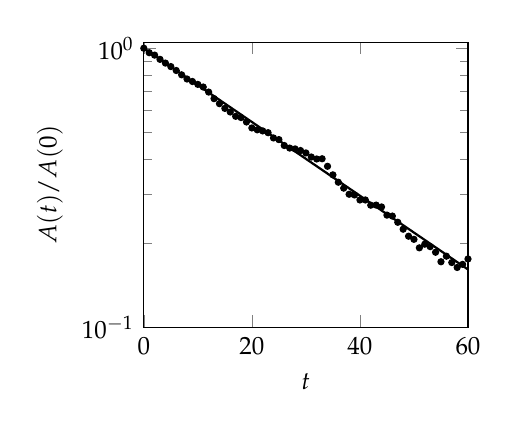
\begin{tikzpicture}
\begin{semilogyaxis}[width=0.47\textwidth,height=5.2cm,
  xlabel={$t$}, ylabel={$A(t)/A(0)$}, ymin=0.1, ymax=1.05, xmin=0, xmax=60,
  tick label style={font=\small}, label style={font=\small}]
\addplot[only marks, mark=*, mark size=1.1pt] coordinates { (0,1.0000) (1,0.9638) (2,0.9448) (3,0.9124) (4,0.8846) (5,0.8596) (6,0.8321) (7,0.8029) (8,0.7758) (9,0.7600) (10,0.7422) (11,0.7261) (12,0.6965) (13,0.6597) (14,0.6329) (15,0.6087) (16,0.5909) (17,0.5701) (18,0.5642) (19,0.5441) (20,0.5179) (21,0.5100) (22,0.5055) (23,0.4981) (24,0.4770) (25,0.4705) (26,0.4480) (27,0.4387) (28,0.4357) (29,0.4299) (30,0.4215) (31,0.4075) (32,0.4010) (33,0.4017) (34,0.3775) (35,0.3517) (36,0.3310) (37,0.3152) (38,0.2997) (39,0.2980) (40,0.2859) (41,0.2859) (42,0.2738) (43,0.2740) (44,0.2699) (45,0.2523) (46,0.2503) (47,0.2378) (48,0.2246) (49,0.2120) (50,0.2066) (51,0.1926) (52,0.1985) (53,0.1945) (54,0.1857) (55,0.1717) (56,0.1798) (57,0.1706) (58,0.1638) (59,0.1680) (60,0.1757) };
\addplot[domain=0:60, samples=2, thick] {exp(-0.03042*x)};
\end{semilogyaxis}
\end{tikzpicture}\hfill
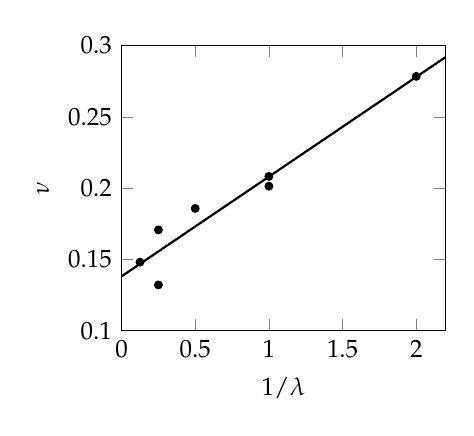
\begin{tikzpicture}
\begin{axis}[width=0.47\textwidth,height=5.2cm,
  xlabel={$1/\lambda$}, ylabel={$\nu$}, xmin=0, xmax=2.2, ymin=0.1, ymax=0.3,
  tick label style={font=\small}, label style={font=\small}]
\addplot[only marks, mark=*, mark size=1.4pt] coordinates { (2,0.2784) (1,0.2013) (1,0.2082) (0.5,0.1857) (0.25,0.1706) (0.25,0.1320) (0.125,0.1480) };
\addplot[domain=0:2.2, samples=2, thick] {0.070*x + 0.138};
\end{axis}
\end{tikzpicture}
\caption{Left: the averaged shear wave at $\lambda=8$ with its fitted
exponential. Right: $\nu$ against $1/\lambda$, with the least-squares line
$\nu=\alpha/\lambda+\beta$.}
\label{fig:viscosity}
\end{figure}

\begin{finding}[E5, E6, viscosity]\label{find:visc}
Table~\ref{tab:viscosity} and Figure~\ref{fig:viscosity}. The viscosity falls
from $0.278$ at $\lambda=\tfrac12$ to $0.148$ at $\lambda=8$. A least-squares
fit gives
\[
\nu \;=\; \frac{\alpha}{\lambda} + \beta,
\qquad \alpha = 0.070,\quad \beta = 0.138,
\]
with largest residual $0.024$. Replicates with fresh seeds (E6) put the standard
error of a single row at $0.023$--$0.027$ for $\lambda=1$, $0.010$ for
$(f,w_2)=(2,2)$ and $0.005$ for $(4,1)$.
\end{finding}

The $1/\lambda$ term is the kinetic-theory term: the viscosity of a gas is
proportional to its mean free path, and the mean free path is inversely
proportional to the collision rate, which the kernel's cross-section sets. The
constant $\beta$ remains as $\lambda\to\infty$ and is a contribution of the
lattice and of asynchronous streaming; it is not derived here, and it is large
--- at the collision parameters reachable in this study it dominates. Whether
$\nu$ depends on $w_2$ and $f$ only through $\lambda$ is a sharper test. At
$\lambda=1$ the two ways of reaching it agree within error
($0.201$ and $0.208$; replicates $0.225$ and $0.194$). At $\lambda=4$ they do not:
the denser gas is less viscous ($0.132$ against $0.171$; replicates $0.153$
and $0.179$), a difference of about two standard errors in each pair. The density
therefore enters through the lattice term as well, and Maxwell's
density-independence of the dynamic viscosity (mass density times $\nu$) is not reproduced
by this model at this precision. The viscosity \emph{is} a property of the
collision kernel --- without the three-body term the mode does not relax at
all, and with it the viscosity moves with the cross-section --- but the model
is a lattice gas, and the lattice has a say.

%==============================================================================
\section{What is shown, what is not, and what is open}\label{sec:status}
%==============================================================================

\paragraph{Shown.} The kernel calculus $\krho$ with the canonical kernel;
COMM as its one-body rule and \rhoc{} as its ideal gas
(Proposition~\ref{prop:ideal}); the virial series of site propensities
(Proposition~\ref{prop:virial}); the shape criterion
(Proposition~\ref{prop:shape}) and mass at the pattern
(Proposition~\ref{prop:mass}); the translation back to \rhoc{} and its
correspondence with the kernel once the fibre multiplicity is included
(Theorem~\ref{thm:corr}, with a proof sketch and Finding~\ref{find:e1});
identity at zero cross-section (Proposition~\ref{prop:identity}); the line
invariants of the two-body lattice kernels (Proposition~\ref{prop:lines}).

\paragraph{Measured, not proved.} The Lindemann fall-off; the decay of the
shear wave and the dependence of the viscosity on the collision parameter.
These are statements about finite simulations, with the finite-size and
statistical caveats that implies.

\begin{obligation}[A full proof of correspondence]\label{ob:corr}
Theorem~\ref{thm:corr} is stated at a site and proved by a counting argument.
The operational correspondence for whole terms --- completeness and soundness up
to administrative steps on locks and up to garbage, together with weight
preservation on the jump chain --- remains to be written out, including the
persistent case in which each firing allocates a fresh lock by $\Frsh$.
\end{obligation}

\begin{obligation}[Emergent geometry]\label{ob:geometry}
The lattice gas takes its geometry from the site names. The aim stated in
Section~\ref{sec:path} is a geometry grown from interaction, with distance a
statistic of the dynamics. The construction of this note supplies the
ingredients --- collisions are three-party events, and bonds formed by
association are persistent edges of the interaction graph --- but not the
self-reinforcement that would make the interaction graph settle into a
low-dimensional geometry rather than randomise into an expander. Measuring its
spectral dimension as a function of the structural rate is the first
experiment to run.
\end{obligation}

\begin{obligation}[Turbulence]\label{ob:turbulence}
Turbulence needs a high Reynolds number $UL/\nu$: small viscosity, which the
kernel supplies by a large collision parameter, together with a forcing and a
system large enough for an inertial range. The asynchronous, exclusion-free
FHP of this note is a starting point; its isotropy and the absence of further
spurious invariants should be checked before it is driven.
\end{obligation}

\begin{obligation}[The dual overlap]\label{ob:dual}
Two receipts contending for one datum is the second critical-pair shape. Its
collision is a collision of contexts, $R\coll S$ filled by one term. The
canonical-kernel construction should extend to it, presumably by matching a
composite pattern against a single payload.
\end{obligation}

\begin{obligation}[Detailed balance and re-bonding]\label{ob:balance}
Association and dissociation are separate laws, not inverse ones, so detailed
balance holds only if their weights are tied deliberately. The relation
between collision-formed bonds and the unbreakable bonds of restriction, and
whether breaking the latter by exposure to its \rhoc{} image belongs in the
same kernel, is open.
\end{obligation}

\begin{obligation}[Bound and collided]\label{ob:bound}
Remark~\ref{rem:bound}: should the pattern language acquire a collision
constructor, so that a receiver can distinguish a pre-bonded molecule from a
collision complex?
\end{obligation}

\begin{obligation}[The coherent case]\label{ob:coherent}
Under $\V=\Cx$ the one-body and many-body branches interfere. Whether that
interference is a defect or the beginning of a scattering theory with
amplitudes, connecting to the permanent of the quantum note, is open.
\end{obligation}

%==============================================================================
\section{Conclusion}\label{sec:conc}
%==============================================================================

A race in the \rhoc{} calculus is a critical pair whose peak is never joined.
Naming the peak gives collision: both bidders arrive, and what happens next is
a substitution into the holes of the receiver. With destructuring patterns the
substitution is canonical --- the receiver's pattern matched against the
composite of the arrivals --- and the many-body terms of that construction are
the virial corrections to an ideal gas that the \rhoc{} calculus, read as a
chemistry, has always been. The receiver's pattern decides whether it can
collide, its cross-section whether it does, and the map back to \rhoc{} is a
lock, a family of self-joins and a weight that counts outcomes rather than
derivations. In a lattice gas built this way, viscosity is produced by the
kernel, and the kernel's two-body term alone does not produce it everywhere.

%==============================================================================
\appendix
\section{The computations}\label{app:comp}
%==============================================================================

All numbers are produced by \texttt{collide.py} (Python 3 standard library
only). \texttt{python3 collide.py e1 e2 e3 e4 e5} reproduces them; seeds are
fixed.

\begin{description}[style=nextline]
\item[E1 (kernel = translation).] Random sites: two to four messages of one or
two atoms over \{a,b,c\}; patterns with up to two constants and up to two
process variables; $w_1,w_2\in[0.2,2]$, $w_3\in[0,1]$; clause
$g(\sigma)=\prod_v(1+\tfrac14|\sigma(v)|)$. The kernel enumerates $k$-subsets
and AC matches; the translation enumerates orderings, splits and per-component
matches, recombines, and weights by $w_kg$, $w_kg/k!$ or $w_kg/\mu$, with $\mu$
computed by an independent contingency-table recursion.
\item[E2 (ideal gas).] Kernel with $w_{k\geq2}=0$ against graded \rhoc{} on
$2{,}000$ random sites; Tables~\ref{tab:virial} and~\ref{tab:jump}.
\item[E3 (propensity tables).] The generic enumerator against the closed-form
propensities used by the fast simulators of E4 and E5, on $400$ random site
configurations.
\item[E4 (Lindemann).] Exact stochastic simulation of the four laws;
$k_{\mathrm{uni}}$ estimated as decompositions divided by the time integral of
$n_A$.
\item[E5 (lattice gas).] Exact stochastic simulation with Fenwick-tree
selection over cells (streaming) and sites (collisions); $L=16$, $a=\tfrac12$,
$h=1$, $T=60$, six independent runs per point, averaged before fitting.
$\Gamma$ is the least-squares slope of $\log A(t)/A(0)$ over the window in
which the averaged ratio exceeds $0.2$, and $\nu=\Gamma/k^2$ with
$k = 2\pi/(L\sqrt3/2)$, the wavenumber of the mode in Cartesian coordinates.
\end{description}

%==============================================================================
{\raggedright
\begin{thebibliography}{99}
%==============================================================================

\bibitem{CF} L.~G.~Meredith.
Choice principles as graded where-clauses.
F1R3FLY.io working note, \texttt{choice-types}, August 2026.

\bibitem{FHP} U.~Frisch, B.~Hasslacher and Y.~Pomeau.
Lattice-gas automata for the Navier--Stokes equation.
\emph{Phys. Rev. Lett.} 56(14):1505--1508, 1986.

\bibitem{FHP87} U.~Frisch, D.~d'Humi\`eres, B.~Hasslacher, P.~Lallemand,
Y.~Pomeau and J.-P.~Rivet.
Lattice gas hydrodynamics in two and three dimensions.
\emph{Complex Systems} 1:649--707, 1987.

\bibitem{Gardiner} C.~W.~Gardiner.
\emph{Handbook of Stochastic Methods}. Springer, 1985.

\bibitem{Gillespie} D.~T.~Gillespie.
Exact stochastic simulation of coupled chemical reactions.
\emph{J. Phys. Chem.} 81(25):2340--2361, 1977.

\bibitem{GW} L.~G.~Meredith.
Graded where-clauses.
F1R3FLY.io working note, \texttt{fuzzyware}, 2026.

\bibitem{GWQ} L.~G.~Meredith.
Races decided by the Born rule.
F1R3FLY.io working note, \texttt{fuzzyware}, version 6, August 2026.

\bibitem{Graphity} T.~Konopka, F.~Markopoulou and L.~Smolin.
Quantum graphity. arXiv:hep-th/0611197, 2006.

\bibitem{HiC} E.~Lieberman-Aiden et al.
Comprehensive mapping of long-range interactions reveals folding principles of
the human genome. \emph{Science} 326(5950):289--293, 2009.

\bibitem{Hinshelwood} C.~N.~Hinshelwood.
On the theory of unimolecular reactions.
\emph{Proc. R. Soc. Lond. A} 113:230--233, 1926.

\bibitem{HPP} J.~Hardy, Y.~Pomeau and O.~de Pazzis.
Time evolution of a two-dimensional model system. I.
\emph{J. Math. Phys.} 14(12):1746--1759, 1973.

\bibitem{KB} D.~E.~Knuth and P.~B.~Bendix.
Simple word problems in universal algebras.
In \emph{Computational Problems in Abstract Algebra}, Pergamon, 263--297, 1970.

\bibitem{Lindemann} F.~A.~Lindemann.
Discussion on ``the radiation theory of chemical action''.
\emph{Trans. Faraday Soc.} 17:598--606, 1922.

\bibitem{Lybech22} S.~Lybech.
Encodability and separation for a reflective higher-order calculus.
EXPRESS/SOS 2022, EPTCS 368, 95--112.

\bibitem{MeredithRadestock} L.~G.~Meredith and M.~Radestock.
A reflective higher-order calculus.
\emph{Electron. Notes Theor. Comput. Sci.} 141(5):49--67, 2005.

\bibitem{NNS} L.~G.~Meredith.
Namespaces without a name server: freshness by communication, and a fully
abstract encoding of the $\pi$-calculus in the rho calculus.
F1R3FLY.io working note, \texttt{pi2rhobugfix}, August 2026.

\bibitem{PLN} L.~G.~Meredith.
Graded where-clauses over the reals.
F1R3FLY.io working note, \texttt{fuzzyware}, August 2026.

\bibitem{Spacetime} L.~G.~Meredith.
Spacetime from cost: a functor from cost-accounted ciGSLTs to measured causal
sets. F1R3FLY.io working note, \texttt{cost-spacetime}, 2026.

\bibitem{UE} L.~G.~Meredith.
Unitary in the equations, measurement in the reductions.
F1R3FLY.io working note, \texttt{fuzzyware}, October 2026.

\bibitem{WGSLT} L.~G.~Meredith.
Weighted graph-structured lambda theories.
F1R3FLY.io working note, \texttt{rho-life}, August 2026.

\end{thebibliography}
}

\end{document}
